\section{FDM, TDM, CDM: algoritmi per la selezione della banda}
\subsection{FDM (Frequency Division Multiplexing) cos'è?}
è una tecnica di condivisione delle risorse trasmissive di un canale di comunicazione. L'intero canale trasmissivo disponibile è diviso in sotto canali, ognuno costituito da una banda di frequenza e separato da un altro grazie ad un piccolo intervallo di guardia.
Questo permette la condivisione dello stesso canale da parte di dispositivi che utilizzano diverse regioni di frequenze e utenti che possono così comunicare contemporaneamente senza interferirsi tra loro.

\begin{figure}[H]
\centering
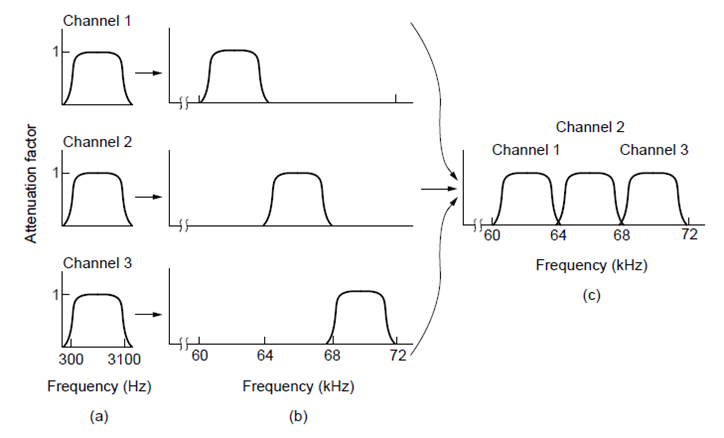
\includegraphics[scale=0.45]{res/img/11_FDM.png}
\end{figure}
\subsubsection{Pregi}
Permette di condividere un intero canale da più utenti, suddividendo le conversazioni in base alle diverse frequenze.
\subsubsection{Difetti}
Gli intervalli di guardia potrebbero essere uno spreco di banda utilizzato unicamente per la sicurezza.
\subsubsection{Ambiti d'uso}
Questa tecnica è comunemente utilizzata nelle trasmissioni televisive, radiofoniche, telefoniche o di dati. Anche le reti cellulari utilizzano in parte questo tipo di multiplazione per suddividere e assegnare l'intera capacità trasmissiva o banda radio disponibile alle varie celle di copertura servite da stazioni radio base.

\subsection{TDM (Time Division Multiplexing) cos'è?}
è una tecnica di condivisione di un canale di comunicazione secondo la quale ogni dispositivo ricetrasmittente ottiene a turno l'uso esclusivo dello stesso per un breve lasso di tempo. Il tempo di utilizzo del canale è diviso in frame tutti della stessa durata, questi frame sono ulteriormente divisi in slot.

\begin{figure}[H]
\centering
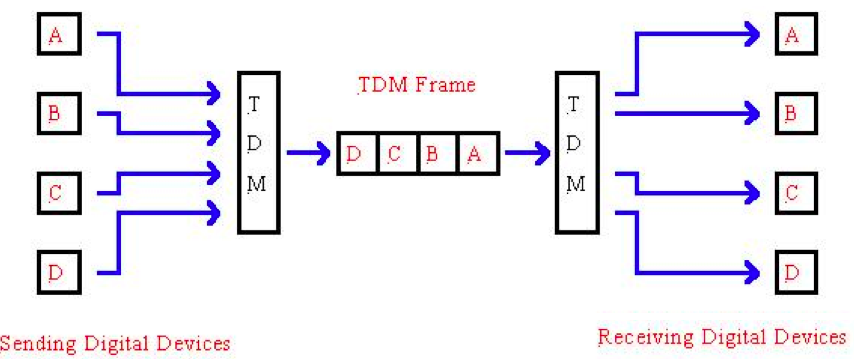
\includegraphics[scale=0.5]{res/img/11_TDM.png}
\end{figure} 

\subsubsection{Pregi}
Più efficiente del FDM in quanto elimina la necessità degli intervalli di guardia.

\subsubsection{Difetti}
Necessita di un circuito di sincronizzazione temporale in ricezione per l'estrazione del time-slot di competenza.

\subsubsection{Ambiti d'uso}
Utilizzata per le trasmissioni di fonia nella rete telefonica. Questo tipo di multiplazione è utilizzata molto nei sistemi a commutazione di circuito.

\subsection{CDM (Code Division Multiplexing) cos'è?}
Conosciuta anche come CDMA è il protocollo di accesso multiplo a canale condiviso. Offre una maggiore velocità di trasmissione di dati rispetto a TDM e FDM.
Questa tecnica è realizzata moltiplicando in trasmissione l'informazione generata per un'opportuna parola detta chip; la sequenza in uscita dal moltiplicatore sarà successivamente modulata e infine trasmessa sul canale.
In ricezione il segnale ricevuto sarà costituito dalla somma vettoriale di tutti i segnali trasmessi dalle singole stazioni. Grazie all'ortogonalità dei chip delle sorgenti, l'estrazione dell'informazione associata a ciascuna sorgente potrà essere fatta moltiplicando il segnale ricevuto con il particolare codice associato alla determinata sorgente che si vuole estrarre.


\begin{figure}[H]
\centering
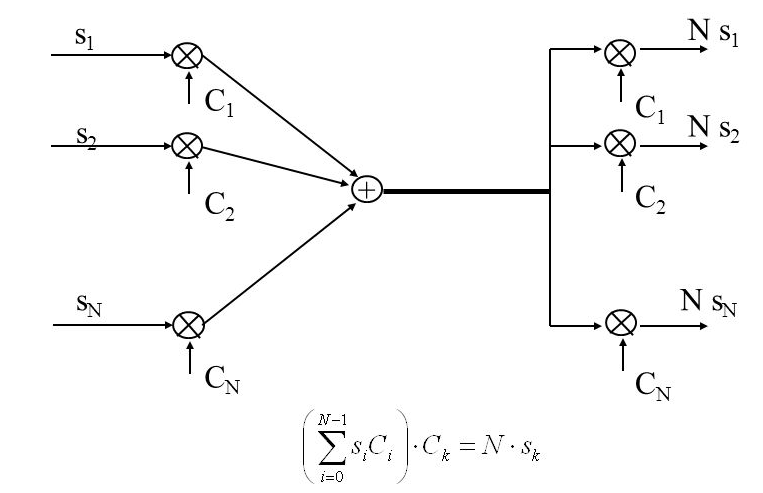
\includegraphics[scale=0.5]{res/img/11_CDM.png}
\end{figure}
\subsubsection{Pregi}
Rispetto a TDM e FDM, CDM garantisce una miglior efficienza dovuta al fatto che ciascun canale utilizza l'intera banda di frequenza assegnata e per tutto il tempo che desidera.
La non-interferenza è assicurata grazie all'uso di codici ortogonali.
Provvede inoltre a fornire una maggior sicurezza dovuta al fatto che i segnali si mescolano nel canale e per estrarne uno è necessario conoscere la parola corretta.
\subsubsection{Difetti}
Necessita di circuiti più complessi rispetto alle altre tecniche di condivisione di un canale.
\subsubsection{Ambiti d'uso}
è il protocollo più diffuso nelle reti wireless e nei dispositivi mobili di seconda generazione e successive.
\section{QAM e QAM16}

QAM è un sistema di modulazione numerica di ampiezza in quadratura, sia digitale che analogica. 
Le portanti sono sinusoidi. Il termine quadratura indica che differiscono di $90^{\circ}$.

Il segnale in ingresso viene suddiviso e modulato per l'ampiezza. Nel caso di segnali digitali, si sommano i segnali modulati e si ottiene una forma d'onda che risulta una combinazione della modulazione di fase e quella d'ampiezza.
Ciascun tipo di modulazione QAM è caratterizzato da un diagramma (costellazione) su cui sono rappresentati tutti gli stati della portante.
La QAM, rispetto alla PSK (Phase shift keying), migliora l'immunità al rumore. 
\subsection{QAM16, cos'è?}
QAM16 non è altro che un tipo di costellazione del QAM, utilizzando quattro ampiezze e quattro fasi, per un totale di 16 diverse combinazioni. Ogni modem ad alta velocità ha un suo schema di costellazione e può comunicare solo con altri modem che adottano lo stesso schema (anche se generalmente un modem riesce a emulare anche quelli più lenti).

\begin{figure}[H]
\centering
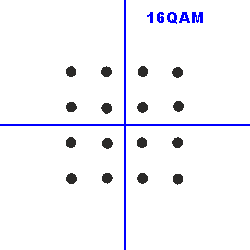
\includegraphics[scale=0.6]{res/img/12_QAM16.png}
\end{figure}

\subsection{Pregi}
Permettono di inviare più bit per baud (simbolo), rispetto alle normali modulazioni. 
\subsection{Difetti}
Ogni modem ha un suo schema a costellazione e può comunicare solamente con altri modem che adottano lo stesso schema.
Questo problema è però in parte ovviato in quanto la maggior parte dei modem è in grado di emulare costellazioni più lente.
\subsection{Ambiti d'uso}
Facente parte dello strato fisico, questo tipo di modulazione è utilizzato come standard per modem telefonici.

\section{byte stuffing?}
Lo strato data link deve servire lo stato network. Per farlo necessita di usare a sua volta le informazioni fornite dallo strato fisico, il cui scopo è quello di prendere un flusso di bit e cercare di portarli a destinazione.
Non esiste nessuna garanzia per la correttezza dei dati, i bit potrebbero essere maggiori, minori, modificati ecc. Uno dei compiti dello strato data link è quello di rilevare ed eventualmente correggere questi errori.
\subsection{Cos'è?}
Il modo per rinvenire questi errori è quello di suddividere il flusso dei bit in frame, per poi controllarli. Uno dei metodi di framing è quello di utilizzare un flag byte con il byte stuffing.

Il byte stuffing prevede l'uso di un flag per delimitare l'inizio e la fine dei frame. In questo modo quando il destinatario perde la sincronizzazione può cercare il flag byte per trovare la fine del frame corrente. Due flag byte consecutivi indicano la fine di un frame e l'inizio del successivo.

Un problema occorre quando vengono spediti dati che per potrebbero replicare il byte FLAG. A questo problema e' stata utilizzata l'implementazione del byte ESC, che precede una occorrenza “accidentale” del byte di FLAG o ESC (in pratica il flag ESC dice di ignorare il successivo byte e prenderlo come byte dati). Successivamente lo strato data link della destinazione provvederà a rimuovere i byte di escape prima di passare i dati allo strato network.


\begin{figure}[H]
\centering
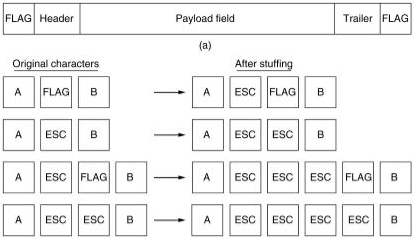
\includegraphics[scale=0.8]{res/img/13_ByteStuffing.png}
\end{figure}

\subsection{Pregi}
Permette una suddivisione di bit in frame tramite l'uso di flag byte, inoltre risolve il problema della sincronia dei frame, grazie ai flag byte che li delimitano.

\subsection{Difetti}
Legato all'uso di caratteri da 8 bit (1Byte): non tutte le codifiche dei caratteri li usano.\\
Per effettuare lo stuffing la quantità di caratteri superflui è notevole.\\
Per risolvere questi problemi è stato creato il bit stuffing.

\subsection{Ambiti d'uso}
Metodo di framing dello strato Data-Link, viene utilizzato in prevalenza dal protocollo PPP per suddividere il flusso di bit in frame.

\section{bit stuffing?}

Lo strato data link deve servire lo stato network, per farlo necessita di usare a sua volta le informazioni fornite dallo strato fisico il cui scopo è quello di prendere un flusso di bit e cercare di portarli a destinazione.
Non esiste nessuna garanzia per la correttezza dei dati, i bit potrebbero essere maggiori, minori, modificati ecc. Uno dei compiti dello strato data link è quello di rilevare ed eventualmente correggere questi errori.
\subsection{Cos'è?}
Per risolvere i problemi e le limitazioni provocate dal byte stuffing, viene sviluppata una nuova tecnica di framing, che prende il nome di bit stuffing, questa nuova tecnica permette di creare data frame che contengono sia un numero arbitrario di frame, sia codifiche di carattere con un numero arbitrario di bit.
Ogni frame comincia e finisce con un gruppo speciale di bit “0111110” (flag byte). Ogni volta che lo strato data link della sorgente incontra cinque “1” consecutivi nei dati inserisce automaticamente un bit con valore 0 nel flusso in uscita. La destinazione quindi quando riceve cinque bit consecutivi con valore 1 seguiti da uno 0, automaticamente elimina lo 0.
Con il bit stuffing il confine fra i due frame viene riconosciuto in modo inequivocabile tramite l'uso della sequenza flag. Inoltre se il ricevente perde traccia dei frame, quello che deve fare e' cercare il byte flag, dato che possono trovarsi sono all'interno del frame e mai all'interno dei dati.

\begin{figure}[H]
\centering
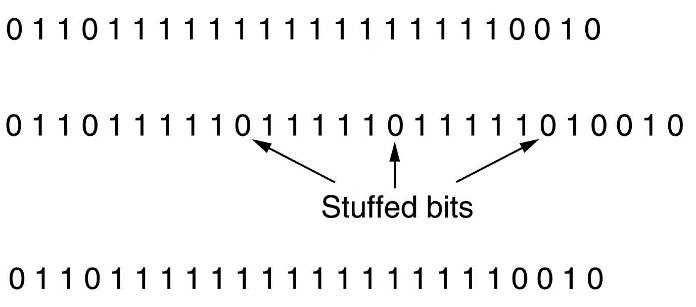
\includegraphics[scale=0.8]{res/img/14_BitStuffing.png}
\end{figure}

\subsection{Pregi}
Risolve i problemi legati dall'uso di 8 bit per il flag byte del suo predecessore (byte stuffing): la poca compatibilità con molte codifiche di caratteri e lo spreco di banda.\\
Permette la suddivisione di bit in frame, facilmente individuabili grazie ai bit flag.

\subsection{Difetti}
--
\subsection{Ambiti d'uso}
Metodo di framing dello strato data link, utilizzato in protocolli che prevedono frame di dimensione fissa: il bit stuffing è utilizzato per raggiungere tale dimensione.\\
Utilizzato anche in alcuni protocolli che prevedono un flusso continuo di dati, gli "0" sono inseriti per assicurare la continuità del flusso.

\section{Numero di bit necessari per riconoscimento (correzione) degli errori di trasmissione?}

I dati trasmessi nei collegamenti locali sono spesso soggetti ad errori, per la loro gestione sono state sviluppate due strategie di base:
la prima si basa su una codifica a correzione d'errore mentre la seconda è una codifica a rilevazione d'errore.
La prima introduce una ridondanza (in ciascun blocco trasmesso) tale da riuscire a ricostruire il messaggio in caso di anomalie.
La seconda invece introduce ridondanza sufficiente solo a capire che c'è stato un errore, ma non di correggerlo.
Un frame generalmente consiste di m bit di dati e r bit ridondanti per i controlli, la somma n=m+r è la lunghezza totale del frame chiamata codeword di n bit.
Date due codeword, per capire quanti bit corrispondenti sono differenti bisogna effettuare l'OR esclusivo e contare il numero di bit a “1” nel risultato,
questo numero è chiamato distanza di Hamming.
\subsection{Bit necessari per rilevare un errore}
Detto questo, per trovare d errori è necessaria una codifica con distanza d+1,
quando la destinazione vede una codeword non valida riesce a determinare che c'è stato un errore, ma non a correggerlo.
\subsection{Bit necessari per rilevare e correggere un errore}
Per correggere d errori è necessaria una codifica con distanza 2d+1,
in tal modo codeword legali sono distanziate in modo tale che anche con d cambiamenti la codeword originale è sempre più vicina di ogni altra,
può quindi essere determinata univocamente.
Un semplice esempio di codifica a rilevazione d'errore si può realizzare aggiungendo un bit di parità ai dati,
calcolato in modo che il numero di “1” nella codeword sia sempre pari (o dispari).
Entrambe le codifiche trovano uso in diversi ambienti.

\subsection{Pregi}
Rilevare semplicemente l'errore permette di diminuire la quantità di bit dati.
Tuttavia rilevazione e correzione permette un minor numero di invii, e permette la ricostruzione autonoma del frames.

\subsection{Difetti}
La semplice rilevazione non permette la ricostruzione del dato, la rilevazione e correzione però necessita del doppio dei bit per poter essere attuata.

\subsection{Ambiti d'uso}
Strato data-link.\\
Nelle reti wireless conviene utilizzare una codifica a correzione dell'errore, cosi da ricostruire il messaggio in casi d'errore
(se si dovesse solo rilevare e richiedere un'altro invio, il rischio della presenza di nuovi errori sarebbe alta, quindi conviene usare questa).\\
Nelle LAN invece, in cui gli errori sono più sporadici, è più conveniente utilizzare spesso quella a rilevazione, con conseguente richiesta di re-invio.

\section{Si descriva cos'è il CRC (Cycle Redundancy check). Si calcoli inoltre il CRC di 10011101 usando il polinomio generatore di $x^4+x+1$}

\subsection{Cos'è?}
Il CRC o Cycle Redundancy Check, è un metodo per il calcolo di somme di controllo, serve a individuare errori casuali nella trasmissione di dati
(causati da interferenze, rumori di linea o distorsione).
Non è utile invece nel caso di tentativi intenzionali di manomissione.
Il CRC tratta le sequenze di bit come dei polinomi a coefficienti che possono assumere solo valori “0” o “1”.
Un frame di k bit è visto come una lista di coefficienti per un polinomio con k termini che variano da $x^k-1$ a $x^0$.
Questo polinomio è detto di grado k-1 e il coefficiente più alto è quello più a sinistra del polinomio
(es 110001 ha 6 bit, quindi rappresenta un polinomio di $5^{\circ}$ grado con coefficienti 1,1,0,0,0 e 1: $x^5+x^4+x^0$.

Quando si utilizza una codifica di questo tipo, sorgente e destinazione devono mettersi d'accordo in anticipo su un polinomio generatore G(x).
Che deve avere i bit di ordine più alto e più basso a “1”.
Per poter calcolare il checksum di un frame di m bit, quest'ultimo dev'essere più lungo del polinomio generatore.
L'idea è quella di aggiungere un checksum alla fine del frame in modo che il polinomio rappresentato dal frame con checksum sia divisibile per G(x).
Quando la destinazione riceve il frame con il checksum e prova a dividerlo per G(x).
Se c'è un resto vuol dire che c'è stato un errore di trasmissione.
\subsection{Esempio}
Ora proviamo con l'esempio di un frame 10011101 con polinomio generatore $x^4+x+1$:
Frame: 1 0 0 1 1 1 0 1 
Generatore G(x): 1 0 0 1 1
Il grado di G(x) è 4, aggiungo 4 “0” al frame (ottenendo un nuovo frame M(x)) in modo da poter dividere le due parti ottenendo il resto da sottrarre al M(x).
M(x)= 1 0 0 1 1 1 0 1 0 0 0 0
Effettuo la divisione: 

\begin{figure}[H]
\centering
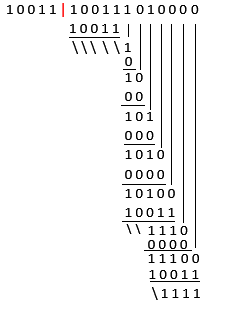
\includegraphics[scale=0.65]{res/img/16_DivisioneEsCRC.png}
\end{figure}
             
1 1 1 1 è il resto di conseguenza, il frame trasmesso è 1 0 0 1  1 1 0 1  1 1 1 1.

\subsection{Pregi}
Richiede conoscenze matematiche modeste, è semplice da realizzare ed ha un ottimo grado di rilevazione degli errori su linee con elevato rumore di fondo.

\subsection{Difetti}
Purtroppo è utile solo per errori causati da interferenze, rumore o distorsione.
L'algoritmo diventa inutile di fronte a tentativi intenzionali di manomissione dei dati.

\subsection{Ambiti d'uso}
Strato data-link.\\
Utilizzato per individuare errori casuali nella trasmissione di dati.
Per i tentativi intenzionali di manutenzione è meglio utilizzare algoritmi di hash quali MD5 e SHA1.

\section{Descrivere il protocollo stop-and-wait, pregi e difetti}

Durante la ricezione dei dati, il frame viene controllato, e a seconda se è integro o meno, si segue uno dei tre diversi protocolli più comuni: 
Stop-and-wait è il più semplice tra questi.
\subsection{Cos'è?}
Un mittente manda solo un frame alla volta, il destinatario, dopo aver ricevuto il frame corretto, invia un ACK (Acknowledge) al mittente, che a sua volta provvede a spedire il secondo frame e cosi via. 
Se l'ACK non raggiunge il mittente, questo provvederà a inviare nuovamente lo stesso frame dopo aver atteso un certo tempo (timeout).
Altri problemi sorgono quando l'ACK arriva danneggiato, in quel caso il mittente invia nuovamente il frame, con il risultato che il destinatario si trova due frame uguali, senza sapere se è un duplicato o se effettivamente il pacchetto successivo ha gli stessi dati, per questo è stato implementato un numero di sequenza per i frame, e il destinatario invia l'ACK inerente a quel frame.
Anche in questo caso sorgono problemi di dissincronia, in cui, sbagliando i numeri dei frame si rischia di perderne molteplici.
Concludendo lo stop-and-wait è parecchio inefficiente rispetto agli altri protocolli di “comunicazione di richiesta di ripetizione automatica”, specialmente a causa del tempo che intercorre tra l'invio dei vari pacchetti e contando anche il fatto che essendoci gli ACK il tempo di comunicazione aumenta considerevolmente, limitando la capacità del canale di comunicazione.
 
\begin{figure}[H]
\centering
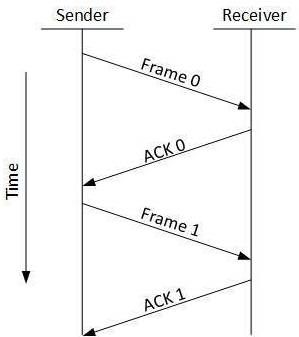
\includegraphics[scale=0.65]{res/img/17_StopAndWait.png}
\end{figure}

\subsection{Pregi}
Permette di gestire i pacchetti ricevuti, corretti o danneggiati, per poi passarli allo strato network.

\subsection{Difetti}
Perdita di dati, lentezza generale, limitato uso del canale di comunicazione.\\
Senza l'utilizzo di piggybacking, o tecniche avanzate, questo protocollo risulta essere estremamente lento e che, a causa della mancata numerazione dei pacchetti, rischia di farne perdere numerosi.


\subsection{Ambiti d'uso}
Strato data-link.\\
Effettivamente questo protocollo non viene utilizzato a causa della parecchia inefficienza rispetto ad altri protocolli.


\section{Cos'è il piggybacking?}

Molti protocolli di comunicazione necessitano di inviare l'ACK come segnale di avvenuta ricezione del frame.
Fatto per ogni singolo frame, questo invio rischia di intasare inutilmente il canale di comunicazione, allungando i tempi e incorrendo in molteplici errori.

\subsection{Cos'è?}
La tecnica del piggybacking permette di aggiungere l'ACK al frame di dati in uscita, utilizzando il campo ack nell'intestazione di questo. In questo modo l'acknowledgement si procura un passaggio gratis insieme al successivo frame dati trasmesso.
Questo avviene quando arriva un frame di dati, la destinazione non invia subito un frame di controllo separato, ma aspetta che lo strato network gli passi il successivo pacchetto.
Un problema può sorgere in caso di attesa molto lunga del pacchetto, poiché si rischia di far scattare il timer del mittente che re-invia il frame nell'attesa dell'ACK, in questo caso si decide un timeout in modo tale da fare piggybacking nel caso in cui il pacchetto da inviare è pronto in tempi celeri, altrimenti si invia l'ACK in modo indipendente.

\subsection{Pregi}
Miglior uso della banda disponibile. E visto che l'ACK viene inglobato nel frame e non inviato singolarmente, la banda viene meno congestionata.

\subsection{Difetti}
In caso di attesa eccessiva del pacchetto dallo strato network, l'ACK potrebbe non venire mai inviato, in quel caso non si attende e si invia l'ACK singolarmente.

\subsection{Ambiti d'uso}
Utilizzato in molti protocolli di comunicazione che necessitano della conferma della ricezione di un determinato messaggio attraverso un ACK. Nelle reti LAN è molto adatta.

\section{Si descriva la tecnica dello Sliding window}
\subsection{Cos'è?}
Sliding window è una classe di protocolli di controllo di flusso di dati.
Una sliding window è formata da una finestra di invio e da una finestra di ricezione.
La prima indica i frame che è autorizzata ad inviare, la seconda invece corrisponde all'insieme dei frame che può accettare.
La finestra di invio contiene i frame da spedire, o spediti ma in attesa di ack, lo scopo è quello di mantenere nel buffer più frame, in modo da ritrasmetterli in caso di problemi. Se questo buffer è pieno, il livello data link costringe il livello network a sospendere la consegna di pacchetti. Quando si ottiene un ack il frame corrispondente esce dalla finestra lasciando posto ad altri.
Analogamente, il destinatario mantiene una finestra corrispondente agli indici dei frame che possono essere accettati, se arriva un frame il cui indice è fuori dalla finestra questo viene scartato (senza invio dell'ack). Se l'indice è dentro la finestra, il frame viene accettato, viene spedito l'ack e si sposta in avanti la finestra.
Le finestre di mittente e destinatario non devono avere necessariamente uguali dimensioni.

\begin{figure}[H]
\centering
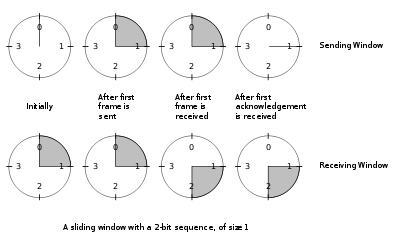
\includegraphics[scale=1]{res/img/19_SlidingWindow.png}
\end{figure}
 
Si noti che nel caso in cui abbiamo una finestra di dimensione massima uguale a 1 ci troviamo nel caso stop-and-wait, ovvero,
dopo aver inviato un frame si attende l'ack corrispondente prima di inviarne ulteriori.
In questo caso si mantiene l'ordine, con finestre più larghe questo non è più vero.

\subsection{Pregi}
Questa classe di protocolli permette di sfruttare al meglio la banda sia in entrata che in uscita, i veri pregi si hanno in base alle dimensioni delle finestre invio/ricezione implementate dai diversi protocolli che sfruttano questa tecnica.

\subsection{Difetti}
--

\subsection{Ambiti d'uso}
Utilizzato prevalentemente dal protocollo TCP nei meccanismi di controllo di flusso e della congestione.

\section{Si descriva l'idea dei protocolli "go back N", indicandone pregi e difetti}

Il problema di ricezione dell'ack per ogni frame inviato, limitava di molto l'utilizzo della banda e rallentava le comunicazioni, per ovviare a questo problema viene usata la tecnica di pipelining. Si decide quindi di inviare più frame prima di ricevere i vari ack aumentando di parecchio l'utilizzo della linea. Tuttavia, sorge un problema, cosa succede nel caso in cui si perdano dei frames? Per il ripristino degli errori in presenza di pipelining sono disponibili due approcci base.Tra questi go back n.
\subsection{Cos'è?}
Go back n è un'istanza specifica del protocollo “Automatic Repeat-reQuest” (modalità di trasmissione di pacchetti di dati) nel quale il processo mittente continua a mandare un numero di frame specificato nella window size anche senza aver ricevuto nessun ACK.
La strategia corrisponde ad una finestra in ricezione di dimensione 1, rilevato l'errore si rifiuta di accettare qualunque frame eccetto il successivo che deve inviare allo strato network. Per questo il mittente scaduto il timeout riprende a spedire i frames che non hanno ricevuto l'ack.
Questa tecnica può essere ottimizzata dall'uso del piggybacking, che consiste nello scrivere l'ack di un pacchetto nell'intestazione del pacchetto di informazione successivo, evitando latenze di trasmissione dovute alla trasmissione del solo ack.
Go back n è uno dei metodi più efficienti per effettuare una connessione in quanto spedisce più pacchetti senza attendere ack, migliorando l'uso della banda, tuttavia può far perdere molta banda se la frequenza degli errori è molto alta.
Go back-n e il selective repeat hanno diverse conseguenze in termini di uso di banda e di spazio di buffer nello strato data link, si può utilizzare un approccio oppure un altro in base a quale risorsa è più scarsa.

\begin{figure}[H]
\centering
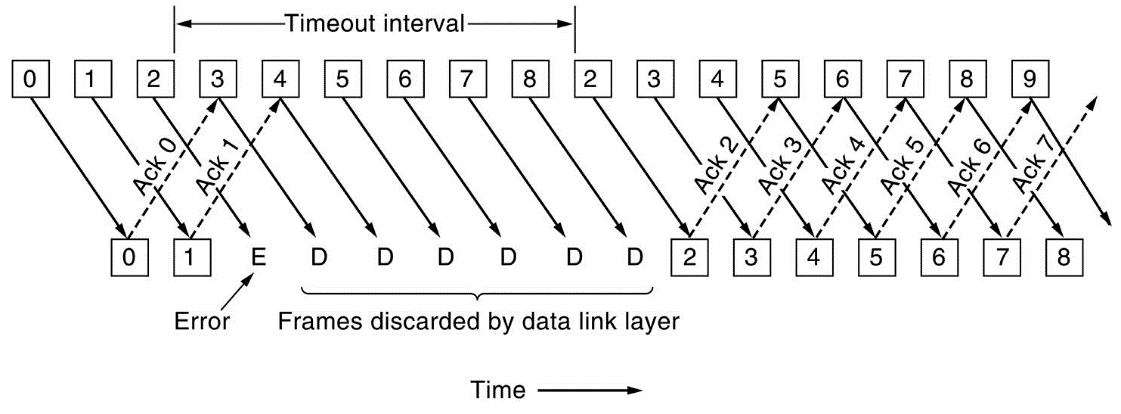
\includegraphics[scale=0.9]{res/img/20_GoBackN.png}
\end{figure}

\subsection{Pregi}
Grazie all'invio a raffica senza attendere l'ack corrispondente, questo protocollo ottimizza in maniera eclatante l'uso della banda (in caso di pochi errori (nulli)).

\subsection{Difetti}
Può far perdere molta banda in caso di un'alta frequenza di errori.

\subsection{Ambiti d'uso}
Viene utilizzato in base alle risorse disponibili, in particolare, nei sistemi in cui la finestra di ricezione è scarsa, e la finestra di invio è più grande.
